Om en funktion $f$ beskriver hur värdet $y$ av någon typ av process beror av en inparameter $x$,
dvs. $y=f(x)$ så beskriver derivatan $f^\prime(x)$ hur snabbt eller långsamt motsvarande process förändras givet indata $x$.
$f^prime(x)$ kan tolkas som förändringshastigheten av $f$ i punkten $x$.

\paragraph{Ex}~\\
$x=$"Framlednings temperatur för radiatorvatten"\\
$f(x)=$"Inomhus temperatur givet framlednings temperatur $x$"\\
$\Rightarrow f^\prime(x)=$ "Förändringshastighet i inomhustemperetaur givet förändring i framledningstemperatur $x$".\\
\\Derivator används och tolkas på liknande sätt i en mängd olika sammanhang för ekonomi/samhällsvetenskap till fysik/teknik/naturvetenskap.

Måste förstå möjligheter, begränsningar och egenskaper för $f^\prime$.

\paragraph{Ex (2.7.20)} Bestäm förändringshastigheten för sidorna av en kub som funktion av kubens volym.
\subparagraph{Lösning} Kalla kubens sidlängd för $s$ och dess volym för $V$.\\
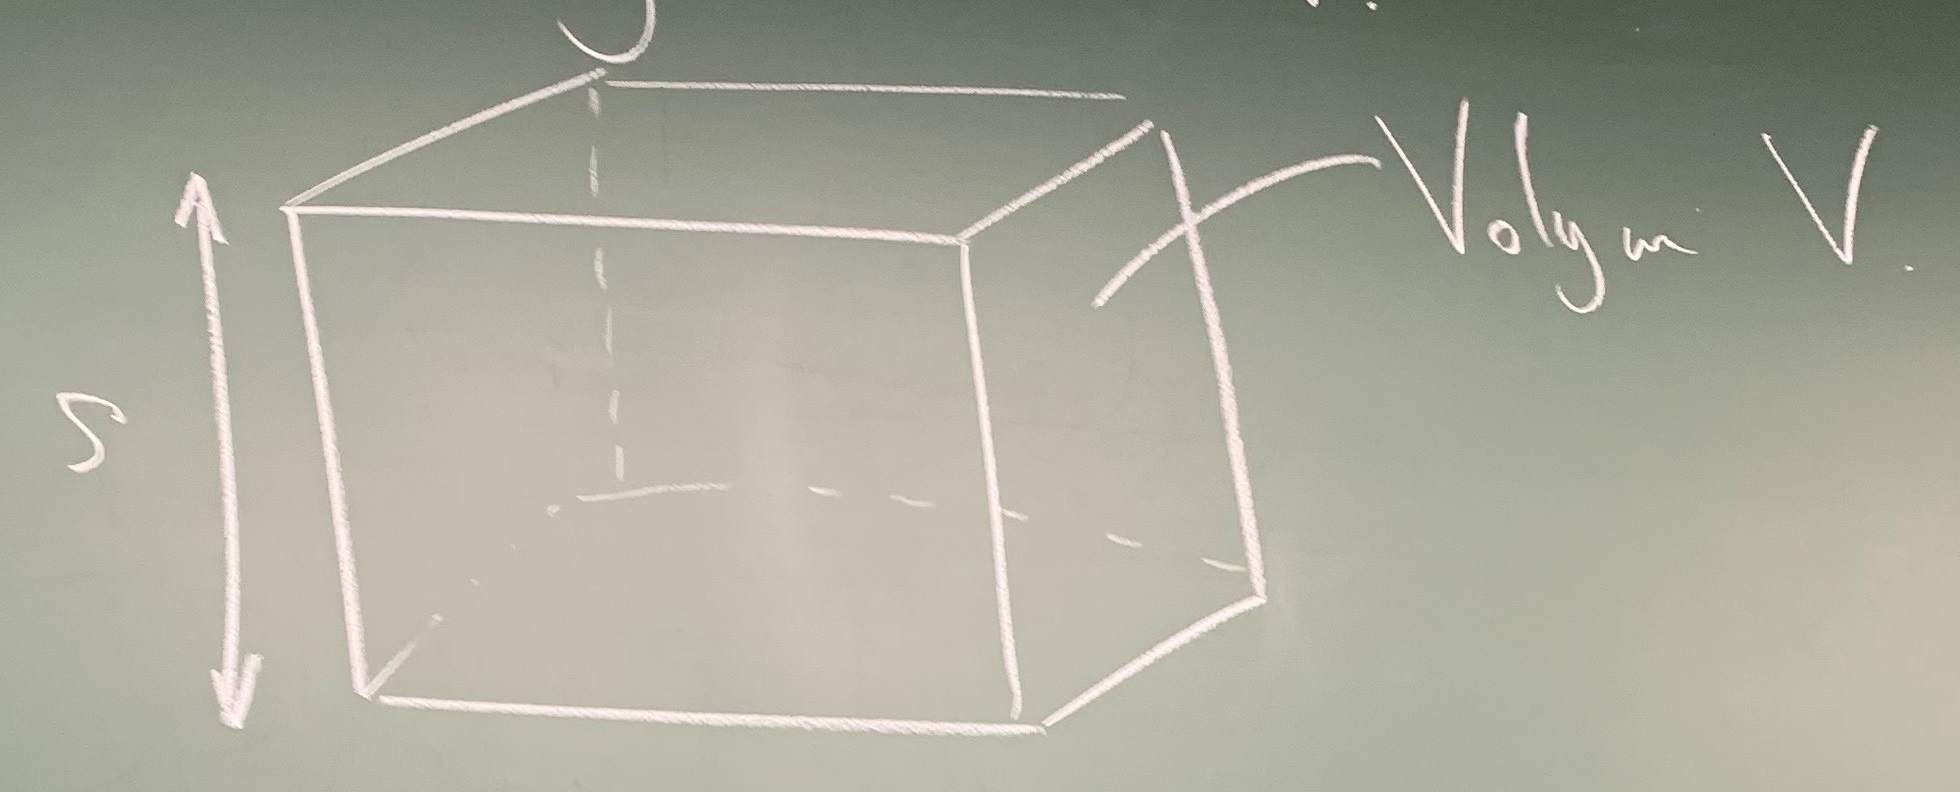
\includegraphics[scale=0.1]{lessons/lesson07/imgs/img01.jpg}\\
Vi villa hitta ett explicit uttryck för $s'(V)$.
Vet att $V=s^3\Leftrightarrow s=\sqrt[3]{V}=V^\frac{1}{3}$.
Alltså är $s'(V)=\frac{1}{3}\cdot V^{\frac{1}{3}-1}=\frac{1}{3}\cdot V=\frac{1}{3\cdot V^{\frac{2}{3}}}$ $\Box$

\paragraph{Ex (2.7.29)} Om det kostar en fabrikör $C(x)$ kr att tillverka $x$ enheter av något så innebär detta en snittkostnad per enhet av $\frac{C(x)}{x}$ (Kr/enhet).
Visa att det antal enheter $x$ som minimerar snittkostnaden gör snitt- och marginalkostnad lika (dvs $C^\prime(x)$).
\subparagraph{Lösning} Låt $A(x)$ beteckna snittkostnad. Dvs. $A(x)=\frac{C(x)}{x}$.\\
Då gäller att:
\begin{equation*}
    A^\prime(x)=\frac{d}{dx}[\frac{C(x)}{x}]=\{\text{prod.reg.}\}=C^\prime(x)\cdot x^{-1}+C(x)\cdot (-1)\cdot x^{-2}=\frac{C^\prime(x)\cdot x-C(x)}{x^2}
\end{equation*}
Vi ser att
\begin{equation*}
    A^\prime(x)=0\Leftrightarrow C^\prime(x)\cdot x-C(x)=0\Leftrightarrow\text{marginalkost.}=C^\prime(x)=\frac{C(x)}{x}=\text{snittkost. }\Box
\end{equation*}
Varför sattes $A^\prime(x)=0$ som en garant för att minimum?
Rent generellt så betyder $f^\prime(x_0)=0$ att en given funktion $f$ har horizontell tangent i $x=x_0$.
Sådana punkter $x=x_0$ kallas för \underline{kritiska punkter} och man säger att $f$ är \underline{stationär} för sådana $x$.
Geometriskt kan detta bara betyda något av följande:\\
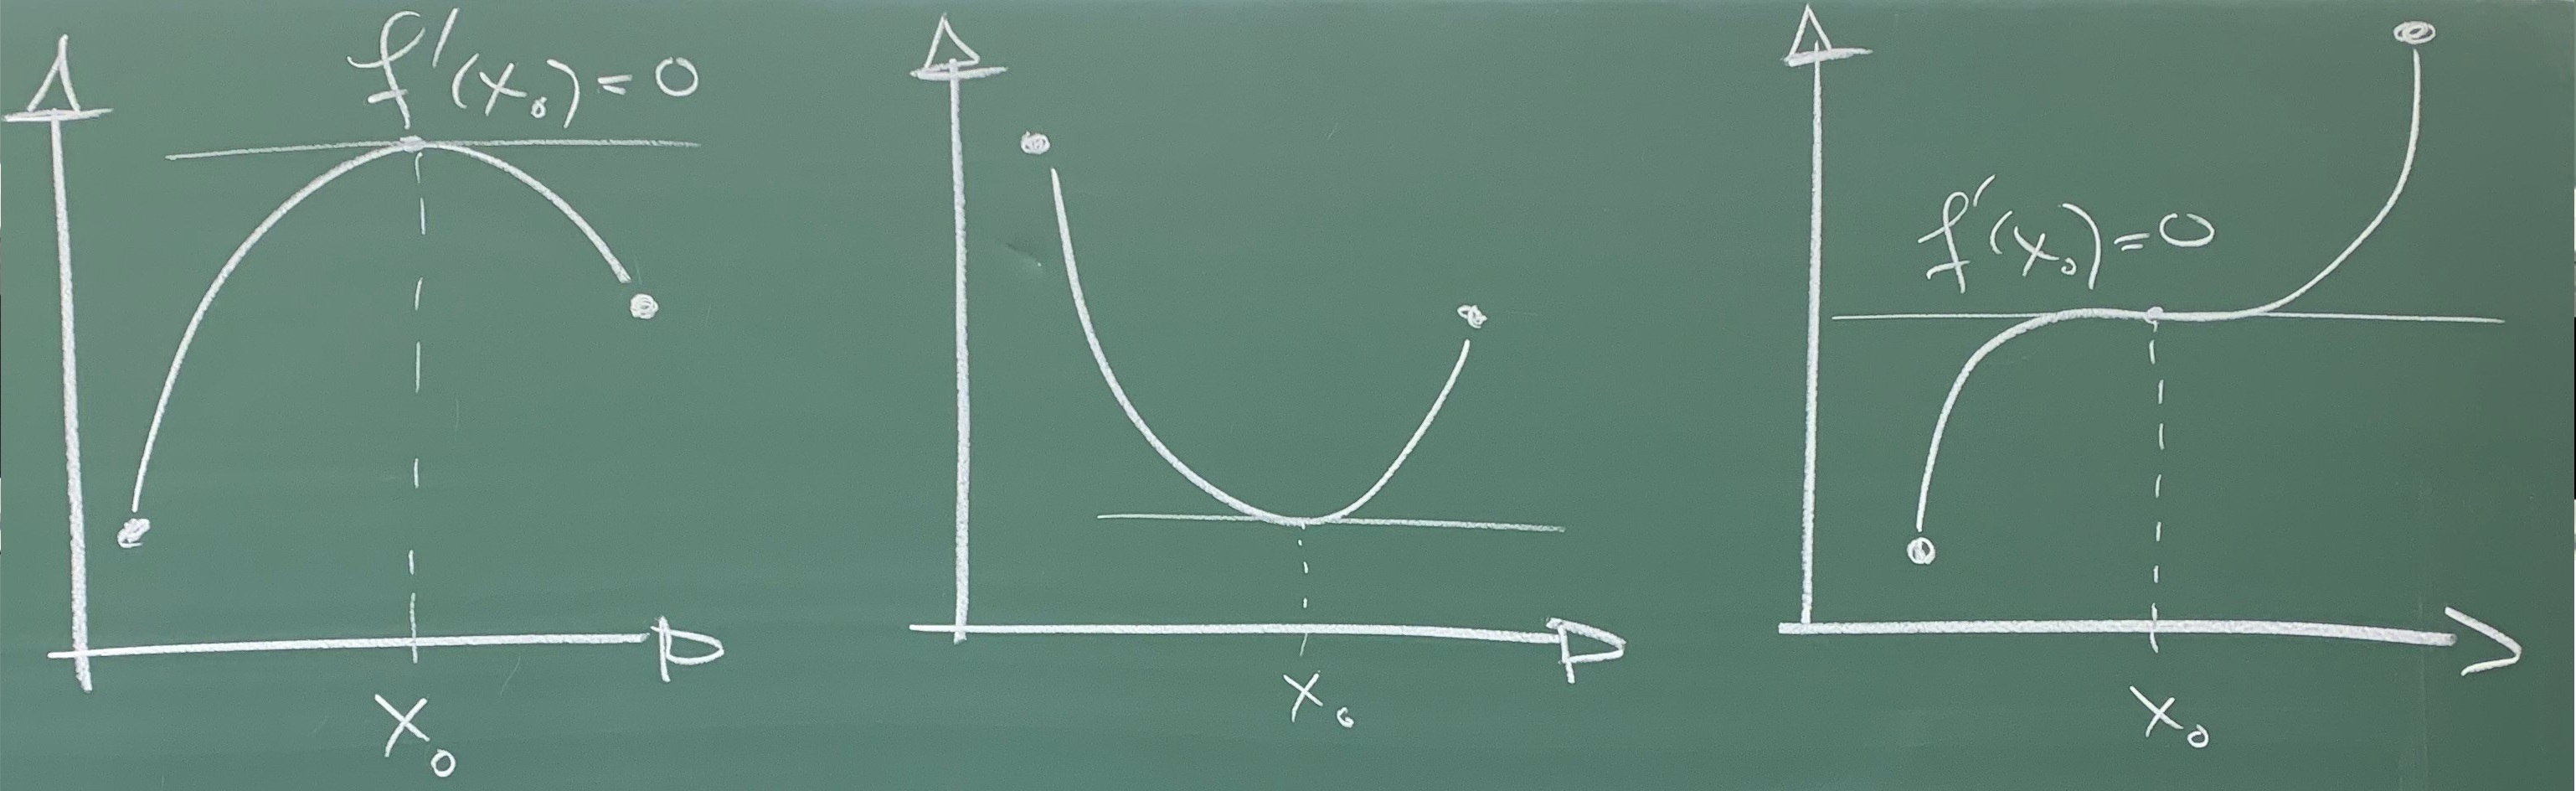
\includegraphics[scale=0.1]{lessons/lesson07/imgs/img02.jpg}\\
Hur visste man att $A^\prime(x)=0$ skulle motsvara en kritisk punkt flr ett minvärde av $A(x)$?
Rimligt att anta att $C(x)=K+c(x)$ där $K$ är en konstant, fast kostand, och $c(x)$ är enhetskostnaden
\begin{itemize}
    \item $A(x)\approx \frac{K}{x}$, om $x$ litet $\Rightarrow$ avtagande.
    \item $A(x)\approx \frac{c(x)}{x}$, om $x$ stort $\Rightarrow$ konstant eller växande.
\end{itemize}
$\Rightarrow A(x)$ har ett minimimum?\\
Smidigt att kika på högre ordning av derivator!\\
Givet en funktion $f$ kan man definiera \underline{andraderivatan} $f^{\prime\prime}$ som $^{\prime\prime}=(f^\prime)^\prime$.
På liknande sätt definieras tredje, fjärde och högre ordnings derivator som $f^{(n)}=((...(f^\prime)^\prime...))^\prime$.
andraderivatan bär precis som förstaderivatan både på teknisk- och geometrisk information om $f$.
Om $x=$tid och $f(x)=$tillryggalagd sträcka så motsvarar $f^\prime(x)$ momentanhastighet och $f^{\prime\prime}(x)$ momentanacceleration.
Geometriskt så kan $f^{\prime\prime}(x_0)$ tolkas som \underline{krökningen} av grafen till $f$ i punkten $x=x_0$.
Det gäller att om
\begin{itemize}
    \item $f^{\prime\prime}(x_0)>0\Rightarrow f$ \underline{konvex} i $x_0$
    \item $f^{\prime\prime}(x_0)<0\Rightarrow f$ \underline{konkav} i $x_0$
    \item $f^{\prime\prime}(x_0)=0\Rightarrow f$ kan vara konvex, konkav eller inget (och kan vara en så kallad \underline{inflektionspunkt}.)
\end{itemize}

Speciellt gäller för stationära punkter där $f^\prime(x_0)=0$ att:
\begin{itemize}
    \item $f^{\prime\prime}(x_0)>0\Rightarrow f$ har ett lokalt minimum i $x_0$
    \item $f^{\prime\prime}(x_0)<0\Rightarrow f$ har ett lokalt maximum i $x_0$
\end{itemize}

\paragraph{Sats} (Rolles sats)\\
Antag att $g$ är konstinuerlig på $[a,b]$ och deriverbar på $(a,b)$.
Om $g(a)=g(b)$ så finns en punkt $c\in(a,b)$ sådan att $g^\prime(c)=0$.
\subparagraph{Notera} Rolles sats är ett specialfall av medelvärdessatsen för derivator.

\paragraph{Sats} (Medelvärdessatsen för derivator) (tenta)\\
Antag att $f$ är en kontinuerlig funktion på $[a,b]$ och deriverbar på $(a,b)$.
Då existerar minst en punkt $c\in(a,b)$ sådan att $\frac{f(b)-f(a)}{b-a}=f^\prime(c)$.\\
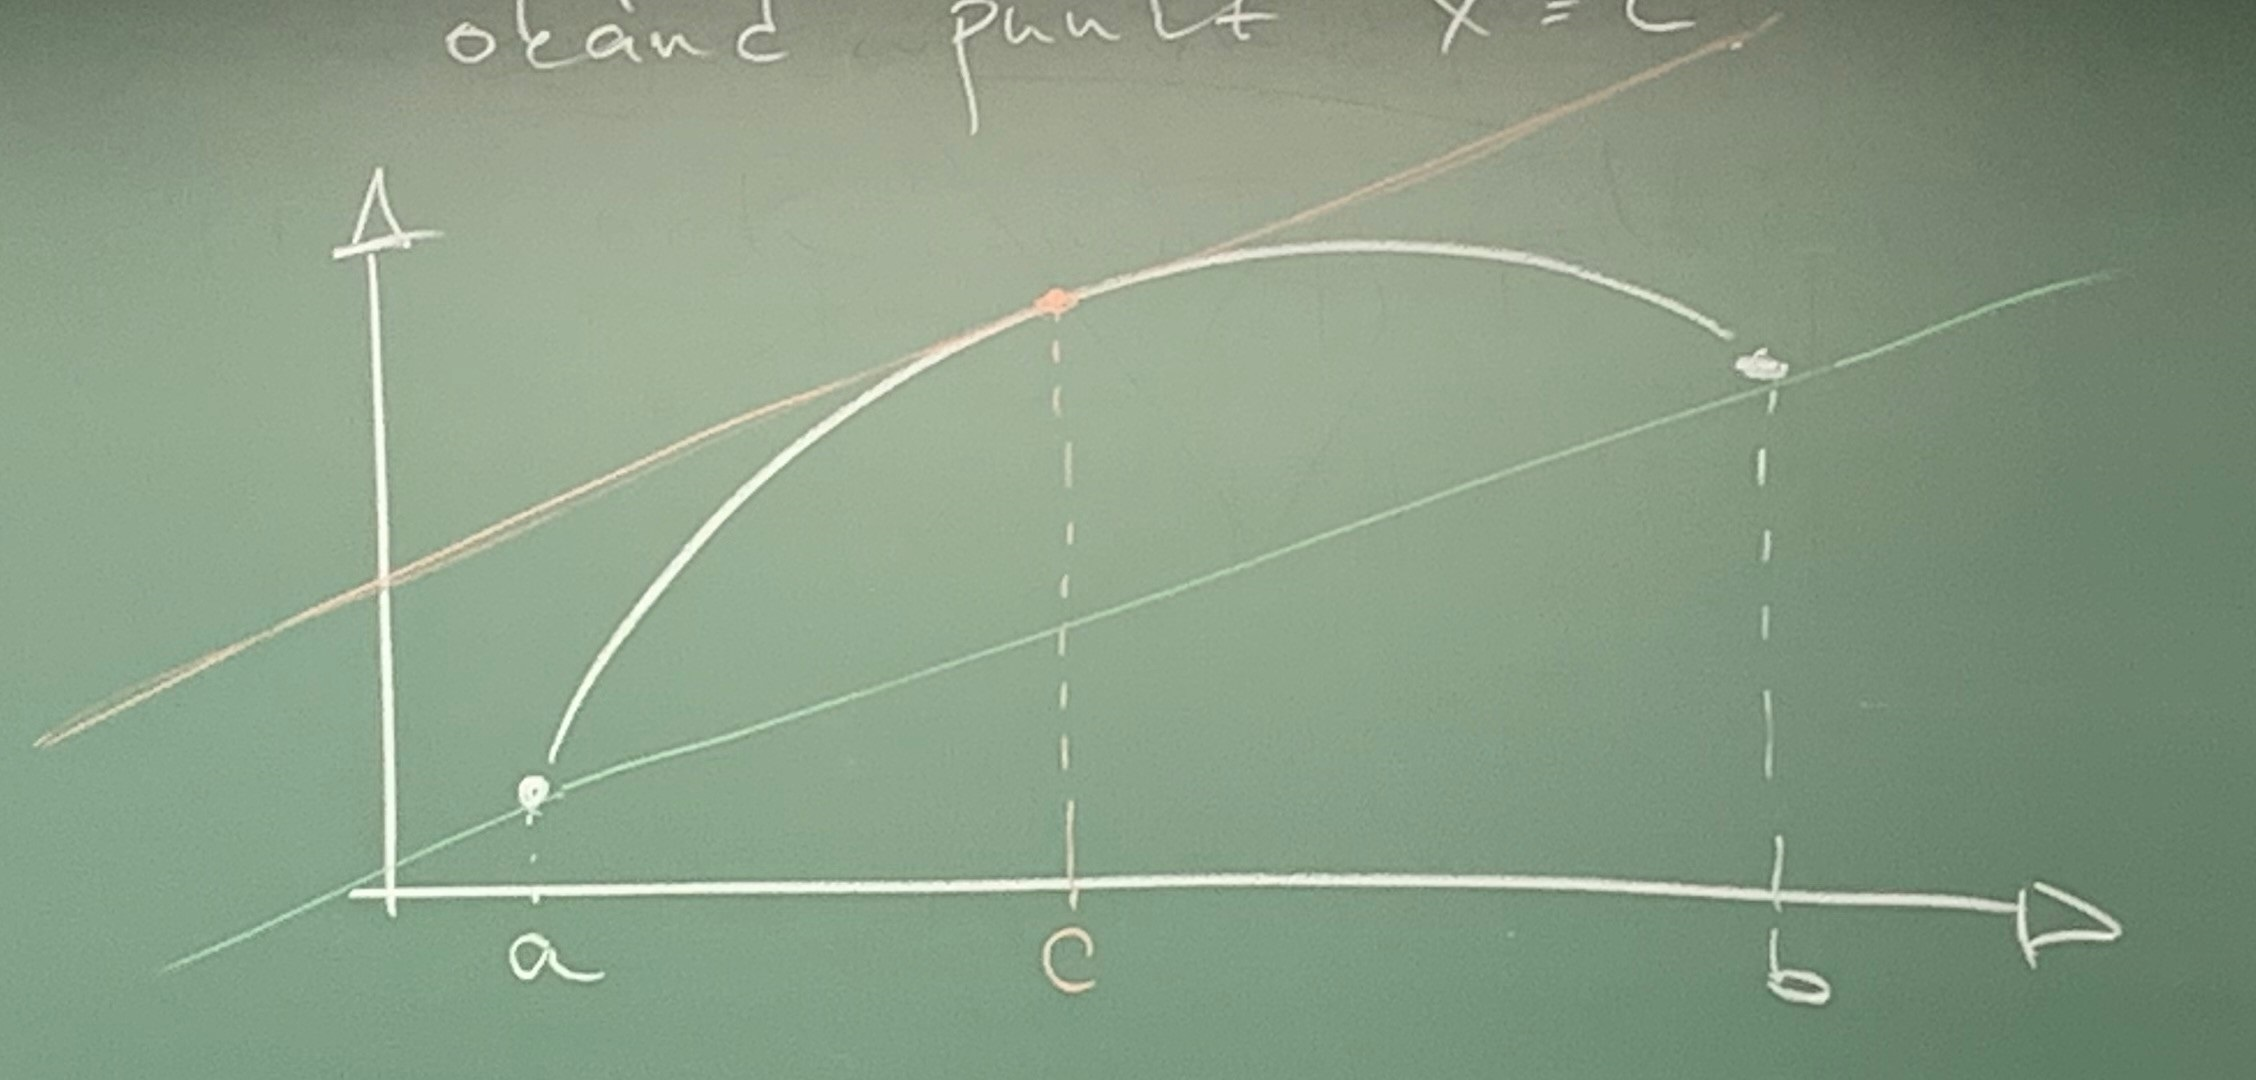
\includegraphics[scale=0.1]{lessons/lesson07/imgs/img03.jpg}\\
\subparagraph{Bevis}
Givet en funktion $f$ som uppfyller villkoren för satsen så kan vi konstruera funktionen $g$ som $g(x)=f(x)-(f(a)+\frac{f(b)-f(a)}{b-a})\cdot (x-a)$.
Uppenbart att $g$ är kontinuerlig på $[a,b]$ och deriverbar på $(a,b)$ då $f$ är det.
Alltså är $g(a)=g(b)$ och $g^\prime(x)=f^\prime(x)-0-\frac{f(b)-f(a)}{b-a}$.
Enligt Rolles sats finns då en punkt $c\in(a,b)$ så att $g^\prime(c)=f^\prime(c)-\frac{f(b)-f(a)}{b-a}$ $\Box$

\paragraph{Sats}
Låt $J$ vara ett öppet intervall och $I$ vara $J$ med eller utan ändpunkter.
Om $f$ är kontinuerlig på $I$ och deriverbar på $J$ gäller att:
\begin{itemize}
    \item $f^\prime(x)\begin{matrix}
                  > \\
                  <
              \end{matrix}\text{ }0\text{, }\forall x\in J \Rightarrow f \begin{matrix}
                  \text{strängt växande} \\
                  \text{strängt avtagande}
              \end{matrix}$ på $I$
    \item $f^\prime(x)\begin{matrix}
                  \geq \\
                  \leq
              \end{matrix}\text{ }0\text{, }\forall x\in J \Rightarrow f \begin{matrix}
                  \text{växande} \\
                  \text{avtagande}
              \end{matrix}$ på $I$
\end{itemize}